% !TEX TS-program = pdflatex
% !TEX encoding = UTF-8 Unicode

% This is a simple template for a LaTeX document using the "article" class.
% See "book", "report", "letter" for other types of document.

\documentclass[11pt]{article} % use larger type; default would be 10pt

\usepackage[utf8]{inputenc} % set input encoding (not needed with XeLaTeX)
\usepackage{amssymb}
%%% Examples of Article customizations
% These packages are optional, depending whether you want the features they provide.
% See the LaTeX Companion or other references for full information.

%%% PAGE DIMENSIONS
\usepackage{geometry} % to change the page dimensions
\geometry{a4paper} % or letterpaper (US) or a5paper or....
% \geometry{margin=2in} % for example, change the margins to 2 inches all round
% \geometry{landscape} % set up the page for landscape
%   read geometry.pdf for detailed page layout information
% \usepackage{amsmath}
\usepackage{graphicx} % support the \includegraphics command and options

% \usepackage[parfill]{parskip} % Activate to begin paragraphs with an empty line rather than an indent

%%% PACKAGES
% \usepackage{booktabs} % for much better looking tables
% \usepackage{array} % for better arrays (eg matrices) in maths
%\usepackage{paralist} % very flexible & customisable lists (eg. enumerate/itemize, etc.)
% \usepackage{verbatim} % adds environment for commenting out blocks of text & for better verbatim
\usepackage{listings}
%\usepackage{subfig} % make it possible to include more than one captioned figure/table in a single float
% These packages are all incorporated in the memoir class to one degree or another...
\usepackage{float}

%%% HEADERS & FOOTERS
\usepackage{fancyhdr} % This should be set AFTER setting up the page geometry
\pagestyle{fancy} % options: empty , plain , fancy
\renewcommand{\headrulewidth}{0pt} % customise the layout...
\lhead{}\chead{}\rhead{}
\lfoot{}\cfoot{\thepage}\rfoot{}

%%% SECTION TITLE APPEARANCE
%\usepackage{sectsty}
%\allsectionsfont{\sffamily\mdseries\upshape} % (See the fntguide.pdf for font help)
% (This matches ConTeXt defaults)

%%% ToC (table of contents) APPEARANCE
%\usepackage[nottoc,notlof,notlot]{tocbibind} % Put the bibliography in the ToC
%\usepackage[titles,subfigure]{tocloft} % Alter the style of the Table of Contents
%\renewcommand{\cftsecfont}{\rmfamily\mdseries\upshape}
%\renewcommand{\cftsecpagefont}{\rmfamily\mdseries\upshape} % No bold!

%%% END Article customizations

%%% The "real" document content comes below...

\title{Travel Buddy - Final Report}
\author{Paul Freeman, Inga Jatzkowski and Diana Hooper}
%\date{} % Activate to display a given date or no date (if empty),
         % otherwise the current date is printed 

\begin{document}
\maketitle
\newpage
%\tableofcontents
%\newpage
\section{Introduction}
The system we are developing is an interactive agent capable of
engaging users in a dialog about travel. The agent will serve as
a travel ``buddy'', by expressing an interest in the travel
experiences of the user, and by talking about the travel
experiences of others. While the primary goal of the agent is
to be engaging to each user, it attempts to achieve the primary
goal by informing the users of experiences they might enjoy,
based on the agent’s beliefs about the users. The purpose is only to provide inspiration for destinations, much like one would often do when conversing about travel. By contrast a travel reccommender system would simply just serve up a reccommendation and that would be it. Our conversation would only halt when the user no longer desires to converse with the agent, again much like how real conversations would end.

\section{Motivation}
Many existing interactive agents are essentially elaborate user
interfaces for case-based reasoning backends or other data retrieval
processes. Additionally, the notion of a basic companion agent has been
extensively researched. Our motivation is to provide a hybrid agent
which provides enjoyable interaction for users while also providing
indirect access to a knowledge base of data on a specific topic.
Because we are not building a travel agent or a complete travel reccommender,
it allows us for more freedom as to what we would like to focus on with our agent. By initially 
creating an agent which can retain simple facts about the user and then relate them to trips 
they might find interesting, coupled with prying information out of the user through simple dialogue, we feel we could have something
that could be a nice proof of concept. Further work could be to add more nuance to the conversation, such as talking about what the user could bring to certain locations or maybe making suggestions based on their possessions.

There will not a be a solution in the form of simply reccommending the perfect trip to the user. Our goal is rather to make a simple emulation of how a conversation about travel would unfold. This agent is able to use its a complex user model and extensive
knowledge base to engage a user in discovering their own solution.
We feel that this approach increases the willingness to interact
with the agent, thus giving more opportunities to solve the problem of getting inspiration for new holiday destinations.

\section{Related Work}
A joint project between researchers in the U.K. and Finland
developed an Embodied Conversational Agent (ECA) to assist
users in planning their day and reminding them to perform
healthy activities. The system works by learning about the
users daily activity by engaging them in everyday conversation.
Rather than requesting specific knowledge from the user, the
conversational approach is more natural for the user, although
it relies on the agent making more inferences on its own. The
beliefs of the system are then used to develop a healthy plan
for each day and the plan is used to make suggestions to the user.

For example, the agent may learn that the user often has free
time before work and suggest to the user that they go to the
gym before work. At the end of the day, the agent will then
follow up and inquire as to whether the user went to the gym
or not. Through this approach, the agent attempts to be less
intrusive in the users life, while still providing a relevant
service in a friendly way.

In an earlier work conducted by a research group in Italy an
Intelligent Travel Recommender (ITR) was developed which used
case-based reasoning to provide the user with suitable
suggestions concerning destination, accommodation and
activities for an upcoming trip. The system uses a very
simple interface for gathering the user’s preferences and
attempts to match their input to its trip databases. In case
of failure, i.e. no matched could be found, it suggests a set
of relaxations to the user’s selected preferences. Additional
to this the system exploits case similarity with older sessions
to rank the results of the user query by computing the
similarities of the items of the current query to those
obtained in similar previous sessions.

The ITR is not a travel agent and doesn’t try to come up
with a conclusive travel plan, it rather suggests suitable
locations, activities, etc. and lets the user collect the
various trip components in their ``travel bag'' for later
review much like a shopping cart at an online shop. 

\section{Analysis}
Our analysis will be broken into several steps. At the
base level, our discovery process will include interviews
with ``experienced travellers''. These people will be used
to gather information for our knowledge base, as well as
provide us with an idea of topics of discussion during a
conversation about travel. Other travel information will
be gathered, as needed, from travel blogs and forums.

Beyond interviews, the analysis process will include a
variety of diagrams showing the interaction of ideas
within our knowledge base. Process diagrams will be used
to layout the order of events the agent moves through
before presenting a response to the user.
Influence diagrams will document information in the
knowledge base that could potentially change beliefs
in other areas. For instance, if the agent adds a belief
that a user dislikes hot weather, this will influence
beliefs about their enjoyment of locations with warm climates.

\section{Design}
\subsection{Overall Architecture}
The Travel Buddy is written in Python and is designed to be
compatible with version 2.7. Porting the code to
Python 3 could be done with little effort. The primary
library at use in the program is PyKE (Python Knowledge
Engine), for which there are version compatible with both
Python 2.6+ and Python 3. As this program is a prototype,
no extra effort has been invested in developing a
user interface. Instead, all I/O is handled through a simple
commandline interface relying on stdin and stdout.

The components of the program can be broken into several
parts, many of which are mandated by the PyKE library.

\subsubsection{Driver}
The driver (implemented in the file driver.py) handles the
basic control flow of a user interaction with the system.
The driver starts the knowledge engine and 
segments the types of interactions available
with the knowledge engine and assists in modelling the
user. Additionally, since PyKE allows forward-chaining to
occur only once for each engine, the driver handles the
creation of multiple engines based on the same knowledge
base in order to facilitate different executions of
forward-chaining rules.

\begin{figure}[H]
\centering
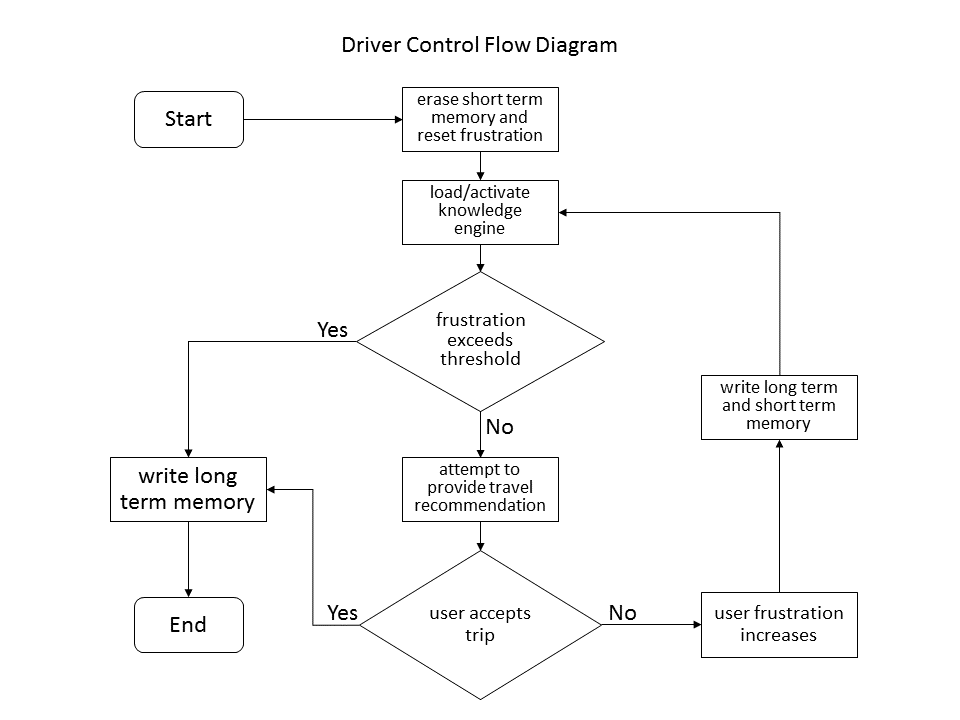
\includegraphics[width=12cm]{driver_control_flow.png}
\caption{Implemented control flow of the main driver.\label{fig:driver}}
\end{figure}

As Figure \ref{fig:driver} shows, the driver begins by erasing the short term memory file and setting the user frustration level to zero. Following these initialization steps, the knowledge engine is activated for the first time. Within the knowledge engine, a number of forward chaining rules run to initialize the session and acquire knowledge about the user. After the completion of the forward chaining rules, the user frustration level is compared to the threshold and the program exits if it is determined the we have been unable to suggest a trip in a reasonable time.

Assuming frustration is within guidelines, the driver attempts to prove a number of backward chaining ``recommenders''. These rules are successfully proved when the knowledge engine finds a trip meeting the recommendation criteria \emph{and} the user indicates they would enjoy the trip. Therefore, if any of the rules can be proved, the program is complete.

If none of the recommenders are proven, the frustration level is increased. Short term memory and long term memory are both writen to disk. The existing knowledge engine is deleted and a new one is created. Recreating the knowledge engine activates the forward chaining rules again, which respond by asking further questions of the user, after which the backward chaining rules again fire. Through this iterative process, the driver attempts to alternate between learning about the user, and suggesting places the user may enjoy. The frustration level guards against boring the user when the Travel Buddy is unable to be useful.

\subsubsection{Memory}
The memory of the Travel Buddy is split into two files, \texttt{shortterm.kfb} and \texttt{longterm.kfb}. Both files are implemented as PyKE Knowledge Fact Base files and, therefore, consist of names attached to tuples of values, where each name/tuple pair represents a piece of knowledge for the system.

The long term memory contains knowledge which is carried over from session to session. It contains facts about users who have previously logged into the system, such as: name, places travelled to, activities enjoyed, weather preferences, and friends. There are also facts about locations and their location within a global hierarchy. The final primary category of facts are those about activities, which specify which locations have certain activities and other minor details.

During each session the system adds appropriate details to the long term memory as facts are learned from the user. For example, if the user answers that they like surfing, the system would record into the long term memory a fact relating the user to enjoying surfing. The long term memory, therefore, contains extensive data about all users who have logged into the system.

The short term memory is used for temporary storage during each session. It contains many different kinds of facts. Certain system facts are stored in short term memory to track from where in the driver code the knowledge engine is being activated. 







The system architecture will be made up out of two main
components. The first part is the knowledge base which contains all the
information about the previous users of the program and
all the trips our ``friend'' knows about. It also contains
the user model that the program keeps of the current
user, which contains all the beliefs about the user’s
travel preferences. And also things that are still unknown
and need to be known for the ``friend'' to make a suitable
recommendation. The other part is the interpretation and
mapping of the user input and the generation of useful
agent output, both in the form of text.

\begin{figure}[H]
\centering
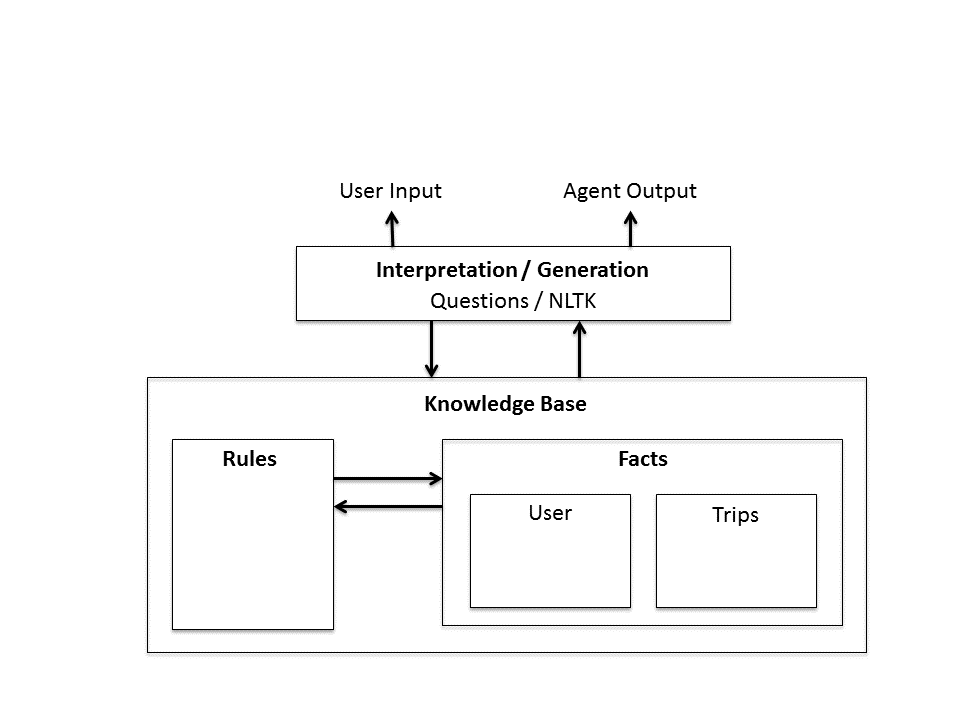
\includegraphics[width=12cm]{architecture.png}
\caption{Proposed design for the overall architecture.}
\end{figure}

The agent itself will be written and designed using the
knowledge engine, PyKE, which is a Python module for logic
programming based on the popular PROLOG language.
PyKE provides us with three kinds of knowledge bases,
the Knowledge Fact Base, the Knowledge Rule Base and
the Knowledge Question Base.

\subsection{Components}

The Knowledge Fact Base will contain all the facts we
know about the user, such as; name, previous trips, travel
possessions, the trips themselves (with associated
locations, weather conditions, interesting sites,
attractions, and activities).

The Rule Base will be used to encode how the program
will make connections between the user’s preferences
stored as beliefs and the trips. It will also try to match
the user to other users in its knowledge base to find
trips that similar users have taken and enjoyed and
recommend them to the current user.

The Question Base can be used to store questions to ask
the user to enquire about their preferences. The
structure of this seems a little inflexible though
upon first impression since we aim for a more natural
feeling dialog than pre-coded questions so the usefulness
of this tool for our system is still up for debate.

A different option for realising a natural language
user dialog is employing the Natural Language Toolkit
(NLTK) for python. NLTK provides different modules
for natural language processing such as lexicons,
parsers or text classification that can be used to
map the user input to a number of discourse acts in
order to extract the relevant information and update
the belief system.

\subsection{Operations}

In order to build a working system, we will need different operations in order to deal with both interpreting the user input, retaining the informations gained from the interpretation and the mapping and then providing some kind of response. For our system we imagine there would be two different kinds of responses, questions and suggesting. Questions have the purpose of directly asking the user in order to clarify things for the user model. Suggestions can be served up as direct suggestions or be formulated as fabricated previous experiences for the agent to which the user can respond positively or negatively, thereby also providing insight to the user's preferences.
We want to present these responses mostly at random in order to avoid making the conversation follow a set pattern.
\\
\\
Our simple interpretation system would work by receiving some user input. Since we are not implementing an extensive natural language processing system, the next step would be to extract known keywords from the input, such as destination names and simple adjectives. Next, we will attempt to extract coherent facts from the keywords and save them to our knowledge base. So if the user inputs "I went to Tahiti. I love Tahiti!"  we save the fact that the user went to Tahiti in our knowledge base and another fact about how they see that destination in a very positive light. If there is some difficulty extracting facts from the keywords, perhaps because of conflicts, we might try to clarify by asking the user directly by presenting what the agent deems the most appropriate interpretation and getting their response. If the user des not accept the interpretation, the agent could try presenting another interpretation or just give a confused response.
\\
The user might also add general information about destinations or their personalities using these adjectives. By saying "I'm very adventurous.", the agent would update its facts by now adding the fact that they are adventurous. Or they could describe a destination as being relaxing or educating, which would in turn add more detail to the descriptions we have of certain trips.
\\
\\
All of these gathered facts are then sometimes used for making suggestions or asking questions. We could for example use the fact that they went to Tahiti and liked it there to look up destinations which share the same characteristics. For this we have a collection of facts about the different destinations. So Tahiti might have a fact categorizing it as being a tropical destination. Doing simple matching, we might just end up pulling another destination which has this fact and suggesting it. During the matching process we will also try to filter out destinations which have characteristics which are seen negatively by the user. We can either completely rule them out or perhaps base our suggestions around a scoring system based on the features, such that some destinations are allowed despite their shortcomings.
\\
\\
Generally the knowledge base is updated updated whenever the agent has an interpretation it is sure of which adds more information. Knowledge is retrieved when making suggestions or asking the user about their experiences or preferences.
\section{References}
%References and such
(1) Marc Cavazza, Cameron Smith, Daniel Charlton, Li Zhang, Markku Turunen, and Jaakko Hakulinen. 2008. A 'companion' ECA with planning and activity modelling. In Proceedings of the 7th international joint conference on Autonomous agents and multiagent systems - Volume 3(AAMAS '08), Vol. 3. International Foundation for Autonomous Agents and Multiagent Systems, Richland, SC, 1281-1284.\\
(2) Ricci, Francesco, et al. "ITR: a case-based travel advisory system." Advances in Case-Based Reasoning. Springer Berlin Heidelberg, 2002. 613-627.\\
(3) Loper, Edward, and Steven Bird. "NLTK: The natural language toolkit." Proceedings of the ACL-02 Workshop on Effective tools and methodologies for teaching natural language processing and computational linguistics-Volume 1. Association for Computational Linguistics, 2002.

\end{document}
